\documentclass[a4paper]{article}

\usepackage[utf8]{inputenc}
\usepackage[margin=0.8in]{geometry}
\usepackage{hyperref,bookmark}
\usepackage{graphicx}
\usepackage{listings}
\usepackage{color}
\usepackage{pdfpages}
\usepackage[style=verbose]{biblatex}
\usepackage{filecontents}
\usepackage[super]{nth}
\usepackage{siunitx}
\usepackage[inline]{enumitem}
\usepackage{listings}
\usepackage{color}
\usepackage[page]{appendix}
\usepackage{cleveref}

\crefname{appsec}{Appendix}{Appendices}

\definecolor{col_light_grey}{rgb}{0.9, 0.9, 0.9}
\definecolor{col_green}{rgb}{0,0.6,0}
\definecolor{col_grey}{rgb}{0.5,0.5,0.5}
\definecolor{col_mauve}{rgb}{0.58,0,0.82}

\lstdefinestyle{none}{
  basicstyle=\footnotesize,
  breaklines=true,
  captionpos=b,
  tabsize=2
}
\lstdefinestyle{default}{
  backgroundcolor=\color{col_light_grey},
  basicstyle=\footnotesize,
  breaklines=true,
  captionpos=b,
  commentstyle=\color{col_green},
  keywordstyle=\color{blue},
  stringstyle=\color{col_mauve},
  tabsize=2
}
\lstset{language=java}

\author{Huw Jones\\27618153\\hcbj1g15@soton.ac.uk}
\title{COMP2208: Intelligent Systems}
\def \subtitle {Comparison of Search Methods}

\def \grid {\textbf{Grid}}
\def \node {\textbf{Node}}

\hypersetup{
  pdfinfo={ee
    Title={\@title},
    Subtitle={\@subtitle}
    Author={\@author},
  },
  colorlinks=false,
  pdfborder=0 0 0,
}

\begin{filecontents}{bib.bib}
\end{filecontents}
\addbibresource{bib.bib}
\pagestyle{headings}

\begin{document}
\makeatletter
\begin{titlepage}
	\centering
	{\scshape\LARGE University of Southampton \par}
	\vspace{2cm}
    {\huge\bfseries \@title \par}
    \vspace{1cm}
	{\scshape\huge \subtitle \par}
	\vspace{3cm}
    {\Large
    \begin{tabular}{c}
      \@author
    \end{tabular} \\}
  \vspace{6cm}
    {\Large
    \today
    }
\end{titlepage}
\makeatother
\newpage

%%
%% SECTION: Approach
%%
\section{Approach}
In order to analyse the differences in scalability, I decided to build a framework that would allow me to minimise the time spent on writing code.
At the moment, I am most familiar with Java, therefore that is the language I chose to build my solution in.
My code is nowhere near ``good'' or optimised (in terms of real time running, not nodes expanded), but it works.

I decided to implement a monitoring thread to print out the current search status.
This means that the number of nodes evaluated, how long the search has been running (in real time), and the amount of memory currently in use.

\subsection{The Setup}\label{sec:approach_setup}
I tried to keep data structures simple and minimalistic.
The state of the puzzle is stored in a \node.
A {\node} has a {\grid} (which represents the state of the puzzle), a parent node reference, a depth (used for IDS), and a priority (used for A*).
A {\grid} has a width/height, a 2D array of characters (representing blocks), and a HashMap that maps characters to their position.

\subsection{The Framework}
I created a framework whereby the program parameters can be manipulated via the command line.
\begin{lstlisting}
-e, --exit [STATE]    Specifies exit state.
-h, --height [HEIGHT] Sets the grid height.
    --help            Prints this help message.
-i, --interval [TIME] Sets the refresh interval (in ms) - for monitoring search status.
-r, --ran [STATE]     Specifies the seed used for the pseudo-random number.
-s, --start [STATE]   Specifies the start state
-t, --type [TYPE]     Specifies the search type:
                      BFS - Breadth First Search
                      DFS - Depth First Search
                      IDS - Iterative Deepening Search
                      A* - A* Heuristic Search
-w, --width [WIDTH]   Sets the grid width.
\end{lstlisting}
This framework allowed me to create scripts to automate my searching.
It also allowed me to inject different start/finish grids, as well as injecting different grid sizes - all without having to rewrite any of my code.

In addition, I allowed the input of the random number seed.
This helped during debugging my program.
If a DFS search didn't work with one random number, I could provide the random number and debug that case.

\subsection{The Organisation}\label{sec:approach_organisation}
My code was organised as following.
All my code is available in \Cref{app:code}.
\begin{lstlisting}
|-- BlocksWorld.java
|-- blocksworld
|   |-- Block.java
|   |-- Grid.java
|   |-- GridController.java
|   |-- Node.java
|   |-- Pair.java
|   |-- Position.java
|   |-- exceptions
|   |   |-- InvalidBlockIDException.java
|   |   |-- InvalidDirectionException.java
|   |   \-- InvalidPositionException.java
|   \-- search
|       |-- AStar.java
|       |-- BFS.java
|       |-- DFS.java
|       |-- IDS.java
|       \-- Search.java
|-- run.sh
\-- test.sh
\end{lstlisting}

I chose to organise my code this way to make it easier for me to add features and group common features together.

\subsection{The Scripts}\label{sec:approach_scripts}
I created a couple of shell scripts to aid my data collection and semi-automate running puzzles.
The most useful script, \texttt{test.sh} (see \Cref{app:code-test}), took a CSV file of puzzle states and executed a given search type on the entire set, then dumped the output to a file.
It saved a long time of running lots of puzzles against all the searches.
\texttt{run.sh} (see \Cref{app:code-run}) is effectively a script that aliases the running of my java program.

%%
%% SECTION: Evidence
%%
\section{Evidence}
A {\grid} state is represented in a grid of dimensions $H \times W$.
The agent is represented by a `\texttt{*}', blanks are represented by `\texttt{-}', and blocks are represented by a lowercase letter.
In the evidence provided, the number above a {\grid} state is the node number.

When a search is running, the current status of the search is displayed.
This include the number of nodes evaluated (time complexity), the length of real time the search has been running, and the amount of used memory (space complexity).

\subsection{Breadth First Search}
\Cref{app:evidence-bfs} shows the order that the program evaluated nodes.
It is evident that BFS is working correctly as the tiles appear to jump around if the nodes are being read in number order.
Here, the first layer of the tree are nodes 1 \& 2.
Nodes 3 to 5 are the second layer children of node 1.
Nodes 6 to 8 are the second layer children of node 2.
Nodes 9 through 11 are the third layer children of node 3.
And so forth for the remainder of the nodes shown.

Example output from a BFS search running is shown in \Cref{app:example-bfs}.
Here, you can see the memory usage, my implementation of BFS fits the expected space complexity.
Since the

\subsection{Depth First Search}
The order of nodes evaluated is shown in \Cref{app:evidence-dfs}.
With these set of nodes, the movement of the agent is fluid from state to state.
Therefore, it can be concluded that the implementation of DFS is working correctly.

\Cref{app:example-dfs} shows the trace of a DFS running.
It shows how few nodes were evaluated (in comparison to BFS), but then the solution is inherently long (compared to the optimal solution).
I think this conclusively proves that my implementation of DFS is working correctly.

\subsection{Iterative Deepening Search}
My implementation of IDS logs when the maximum search depth increases.
In the output log - as shown in \Cref{app:evidence-ids} - it can be seen that the nodes processed follow the expected order for IDS.
When the depth is increased, it is evident that the search restarts again from the root node and proceeds to search down to the maximum depth.

In addition, the memory usage (space complexity), as shown in the output in \Cref{app:example-ids}, seems to follow no trend.
I believe this is due to the nodes on the fringe (at maximum depth) being removed as they aren't a solution.
This would explain why the footprint of IDS stays so small when it is running.

\subsection{A* Heuristic Search}
With A* Heuristic Search, it is more difficult to prove that the algorithm is working correctly.
\Cref{app:evidence-a*} shows the output log for A* Search.
It is more difficult to see how my implementation of A* prioritises its node selection, however, I believe it to be working correctly.
\Cref{app:example-a*} shows that very few nodes were evaluated (compared to other optimal searches such as BFS), and yet the optimal solution was found.

%%
%% SECTION: Scalability
%%
\newpage
\section{Scalability}
I use the term \textbf{complexity} synonymously with difficulty in regards to searching throughout this report.
In this report, the difficulty/complexity number is the length of the optimal solution for a problem.

\paragraph{To investigate the scalability of all 4 searches, I decided to start with the given problem and work backwards.}
The base (given) problem required a minimum of 14 moves to solve and since my searches printed out the list of states to complete the puzzle,
I used this printout to form puzzles of different complexities.
This is how I controlled the ``Problem Difficulty''.

As mentioned in \Cref{sec:approach_scripts}, I wrote a script to automate running puzzles of different complexities.
I used the output from the base puzzle to create a CSV of states to test.
These states ranged from a complexity of 1, to 14 (the base problem).
I ran this test script of all 4 of the search types.

\paragraph{The graph in \Cref{app:graph_4x4} displays my findings.}
It is important to note that I've used a logarithmic scale on the y axis to enhance the readability of the graph.

The most striking element of this graph is how ``random'' the line for DFS is.
This shows that the complexity of DFS is not directly linked to the difficulty of the puzzle.
This is to be expected for DFS as there is no ``real'' logic to how it searches -- it tries random moves until it finds a solution.

The lines for BFS/IDS seem to intertwine and have the same gradient.
Having the same gradient shows that both search methods increase at roughly the same exponential rate (in regards to time complexity against problem difficulty).
There are times where IDS time complexity is less than BFS complexity.
This is most probably due to the location of the solution node.
Since BFS searches left to right, top to bottom and IDS searches from top to bottom, left to right, if the solution is on the bottom left of the tree, IDS will find it before BFS.

Finally, it's important to note how dramatic the difference between A* and BFS/IDS are in terms of time complexity.
With A* the heuristics make all the difference between an efficient search and an inefficient search.
In this investigation, my heuristic function is inadmissible as it is the sum of the Manhattan Distance, Depth of the Node, and the number of blocks in the incorrect position.
With this heuristic function, the time complexity for A* increases exponentially with the problem difficulty, but not to the same extent as that of BFS/IDS.
At a problem with difficulty of ``14'', A* had a time complexity 3 orders of magnitude smaller than BFS/IDS.

\paragraph{Overall, this graph shows the striking difference in time complexities.}
I can safely conclude that the best search method, of the 4 compared, is A* Heuristic Search.
It is evident that using the heuristic function mentioned previously, A* search has a time complexity magnitudes smaller, than that of IDS/BFS.
This effectively rules IDS/BFS out.
DFS, although sometimes providing good time complexity for some random seeds, is ultimately a poor choice if you are wanting to find the optimal solution.


%%
%% SECTION: Extras & Limitations
%%
\section{Extras \& Limitations}

\subsection{Extras}
\subsubsection{Complexity vs Problem Size}
I decided to go a little further whilst investigating the complexity for different problem sizes.
I collected data for puzzles on different grid sizes.
I used grids sized 2x2, 3x3 and 5x5.

The graphs for these grids are available in \Cref{app:graph_2x2}, \Cref{app:graph_3x3}, \Cref{app:graph_4x4}, and \Cref{app:graph_5x5}.

These graphs only reinforce my conclusions in the previous section.

With DFS, the conclusions of randomness and being erratic are shown conclusively.
For example, a problem with difficulty of 1 (1 move to solve the puzzle) took DFS 2,604,225 evaluations to find a solution -- the solution was 2,604,224 moves too long (compared to the optimal solution).
But on the other hand, a problem that took 3.9 million evaluations using A* (as yet to be solved using DFS/IDS), solved by DFS by evaluating only 826,179 nodes.
However, the major caveat being the solution from A* was 21 moves long, and the solution from DFS was 826,179 moves long.

\subsubsection{Space Complexity vs Time Complexity}
In this section, I decided to look at the trends between Time Complexity (number of nodes evaluated) and Space Complexity (indicated by RAM usage).
The graphs are included in the Appendix.
Where a trendline has been plotted, it should in theory have a y-intercept of 0, however, due to the overhead of loaded classes and the JVM, this base usage is in fact approximately 30MB.

\paragraph{BFS Complexity}
The graph in \Cref{app:graph_bfs} shows a fairly linear trend.
As the time complexity increases, the space complexity increases at the same rate.
This is to be completely expected because a Breadth First Search does not allow for nodes to be removed from memory.

\paragraph{DFS Complexity}
The graph in \Cref{app:graph_dfs} shows a linear trend.
As the time complexity increases, the space complexity increases at roughly the same rate.
This graph is not as conclusive due to the massive steps every so often.
However, I attribute this to garbage collection.

To minimise interruptions and reduce CPU usage, garbage collection does not run all the time, but periodically.
There are several measures that are watched and trigger garbage collection;
  these include time intervals, heap size.
In the case of this graph, I believe garbage collection was being trigger when the heap grew too big.
Then garbage collection kicked in and removed a lot of junk (unused/orphaned objects) from the heap.

It is obvious that my implementation of DFS is not optimal, otherwise this memory profile would be less obvious.
Anyway, I believe that this graph shows that the time complexity and space complexity are linearly linked.

\paragraph{IDS Complexity}
The graph in \Cref{app:graph_ids} shows absolutely not trend whatsoever.
Unlike the dodgy garbage collection in the DFS graph (\Cref{app:graph_dfs}) I think garbage collection has worked really well for IDS.

It is noted that the maximum memory usage is 151MB.
This was when IDS had evaluated just over 11 million nodes.
IDS works by searching top to bottom until it reaches a limit, then left to right.
If it does not find a solution, it increases its depth limit and tries again.
Because of this, when IDS hits the limit on the left side of the tree, those nodes are removed from memory as it travels to the right hand side.
This means that IDS has a very small space complexity footprint -- and this is reflected in my findings.

\paragraph{A* Heuristic Complexity}
The graph in \Cref{app:graph_a*} shows a linear trend.
I attribute thickness of the ``line'' to be due to garbage collection -- yet again.

A* works by expanding nodes, evaluating their ``goodness'' (also know as priority), and then expanding nodes from the ``good'' nodes.
This strategy minimises the amount of nodes that are looked at, but means that almost all nodes end up being stored in a Priority Queue.
Therefore, as the number of nodes expanded increases, then the space complexity footprint will also increase.
I strongly believe that my graph shows this to be true.

\subsection{Limitations}
To produce my data for scalability, I only tested 1 grid for each problem difficulty.
If I had more forethought and time, I would've tested the searches against a number of different permutations for each problem difficulty.
This would exclude rotated and reflected puzzles, but would include unique different puzzles.
For example, I only tested the searches against the puzzle labelled A, I would have liked to test against other puzzles with a difficulty of 2 as well -- some examples are shown below.
\begin{verbatim}
A:      B:      C:
----    --*-    ----
-*--    --a-    a---
ba--    -b--    *b--
-c--    -c--    -c--
\end{verbatim}

Although I do not think that testing against different states with the same difficulty would have affected my conclusions, I would still have preferred to use more data.

\paragraph{This report only looked at square grids.}
However, my code did not actually limit the input to have to be square in proportion.
I definitely could have investigated the effect that different sized grids had on the effectiveness of the searches,
  but considering this report's purpose was to compare and contrast the effectiveness of different tree search algorithms, I figured this would have been a little too far out of the scope of the report.
In addition, I don't think that non-square grids would have had any affect on my outcomes -- but that is a claim to be investigated more thoroughly in the future.

\paragraph{Optimal Coding}
I believe I was a bit overambitious whilst trying to investigate 5x5 grids.
Even though A* and DFS could find the solution for a 5x5 with a difficulty of 21, both IDS and BFS could not solve puzzles with a difficulty greater than 15.
I ran the tests on heavy duty servers (with enough resources) for about an hour or so, but each time the search approached using 26GB of RAM (yes, really, 26GB) it seemed to stall completely.
I tried changing servers and tweaking JVM settings, but ultimately, I attribute this limitation to my unoptimised code.

%%
%% SECTION: References
%%
%\section{References}

%%
%% APPENDICES
%%
\newpage
\begin{appendices}
  \bookmarksetupnext{level=-1}
  \addappheadtotoc
  \crefalias{section}{appsec}
  \crefalias{subsection}{appsec}

  %%
  %% SECTION: Code
  %%
  \section{Code}
  \label{app:code}
  \subsection{BlocksWorld.java}
  \label{app:code-BlocksWorld}
  \lstinputlisting[style=default, language=java]{src/BlocksWorld.java}

  \newpage
  \subsection{Grid.java}
  \label{app:code-Grid}
  \lstinputlisting[style=default, language=java]{src/blocksworld/Grid.java}

  \newpage
  \subsection{GridController.java}
  \label{app:code-GridController}
  \lstinputlisting[style=default, language=java]{src/blocksworld/GridController.java}

  \newpage
  \subsection{Node.java}
  \label{app:code-Node}
  \lstinputlisting[style=default, language=java]{src/blocksworld/Node.java}

  \newpage
  \subsection{Pair.java}
  \label{app:code-Pair}
  \lstinputlisting[style=default, language=java]{src/blocksworld/Pair.java}

  \newpage
  \subsection{Position.java}
  \label{app:code-Position}
  \lstinputlisting[style=default, language=java]{src/blocksworld/Position.java}

  \newpage
  \subsection{InvalidBlockIDException.java}
  \label{app:code-InvalidBlockIDException}
  \lstinputlisting[style=default, language=java]{src/blocksworld/exceptions/InvalidBlockIDException.java}

    \subsection{InvalidDirectionException.java}
  \label{app:code-InvalidDirectionException}
  \lstinputlisting[style=default, language=java]{src/blocksworld/exceptions/InvalidDirectionException.java}

  \subsection{InvalidPositionException.java}
  \label{app:code-InvalidPositionException}
  \lstinputlisting[style=default, language=java]{src/blocksworld/exceptions/InvalidPositionException.java}

  \newpage
  \subsection{AStar.java}
  \label{app:code-AStar}
  \lstinputlisting[style=default, language=java]{src/blocksworld/search/AStar.java}

  \newpage
  \subsection{BFS.java}
  \label{app:code-BFS}
  \lstinputlisting[style=default, language=java]{src/blocksworld/search/BFS.java}

  \newpage
  \subsection{DFS.java}
  \label{app:code-DFS}
  \lstinputlisting[style=default, language=java]{src/blocksworld/search/DFS.java}

  \newpage
  \subsection{IDS.java}
  \label{app:code-IDS}
  \lstinputlisting[style=default, language=java]{src/blocksworld/search/IDS.java}

  \newpage
  \subsection{Search.java}
  \label{app:code-Search}
  \lstinputlisting[style=default, language=java]{src/blocksworld/search/Search.java}

  \newpage
  \subsection{run.sh}
  \label{app:code-run}
  \lstinputlisting[style=default, language=bash]{run.sh}

  \subsection{test.sh}
  \label{app:code-test}
  \lstinputlisting[style=default, language=bash]{test.sh}

  %%
  %% SECTION: Output Evidence
  %%
  \newpage
  \section{Output Evidence}
  \subsection{Breadth First Search}
  \label{app:evidence-bfs}
  \lstinputlisting[style=none]{snippets/evidence-BFS.txt}

  %\newpage
  \subsection{Depth First Search}
  \label{app:evidence-dfs}
  \lstinputlisting[style=none]{snippets/evidence-DFS.txt}

  \newpage
  \subsection{Iterative Deepening Search}
  \label{app:evidence-ids}
  \lstinputlisting[style=none]{snippets/evidence-IDS.txt}

  %\newpage
  \subsection{A* Heuristic Search}
  \label{app:evidence-a*}
  \lstinputlisting[style=none]{snippets/evidence-A*.txt}

  %%
  %% SECTION: Example Output
  %%
  \newpage
  \section{Example Output}
  \subsection{Breadth First Search}
  \label{app:example-bfs}
  \lstinputlisting[style=none]{snippets/example-BFS.txt}

  \newpage
  \subsection{Depth First Search}
  \label{app:example-dfs}
  \lstinputlisting[style=none]{snippets/example-DFS.txt}

  \newpage
  \subsection{Iterative Deepening Search}
  \label{app:example-ids}
  \lstinputlisting[style=none]{snippets/example-IDS.txt}

  \newpage
  \subsection{A* Heuristic Search}
  \label{app:example-a*}
  \lstinputlisting[style=none]{snippets/example-A*.txt}

  %%
  %% SECTION: Graphs
  %%
  \newpage
  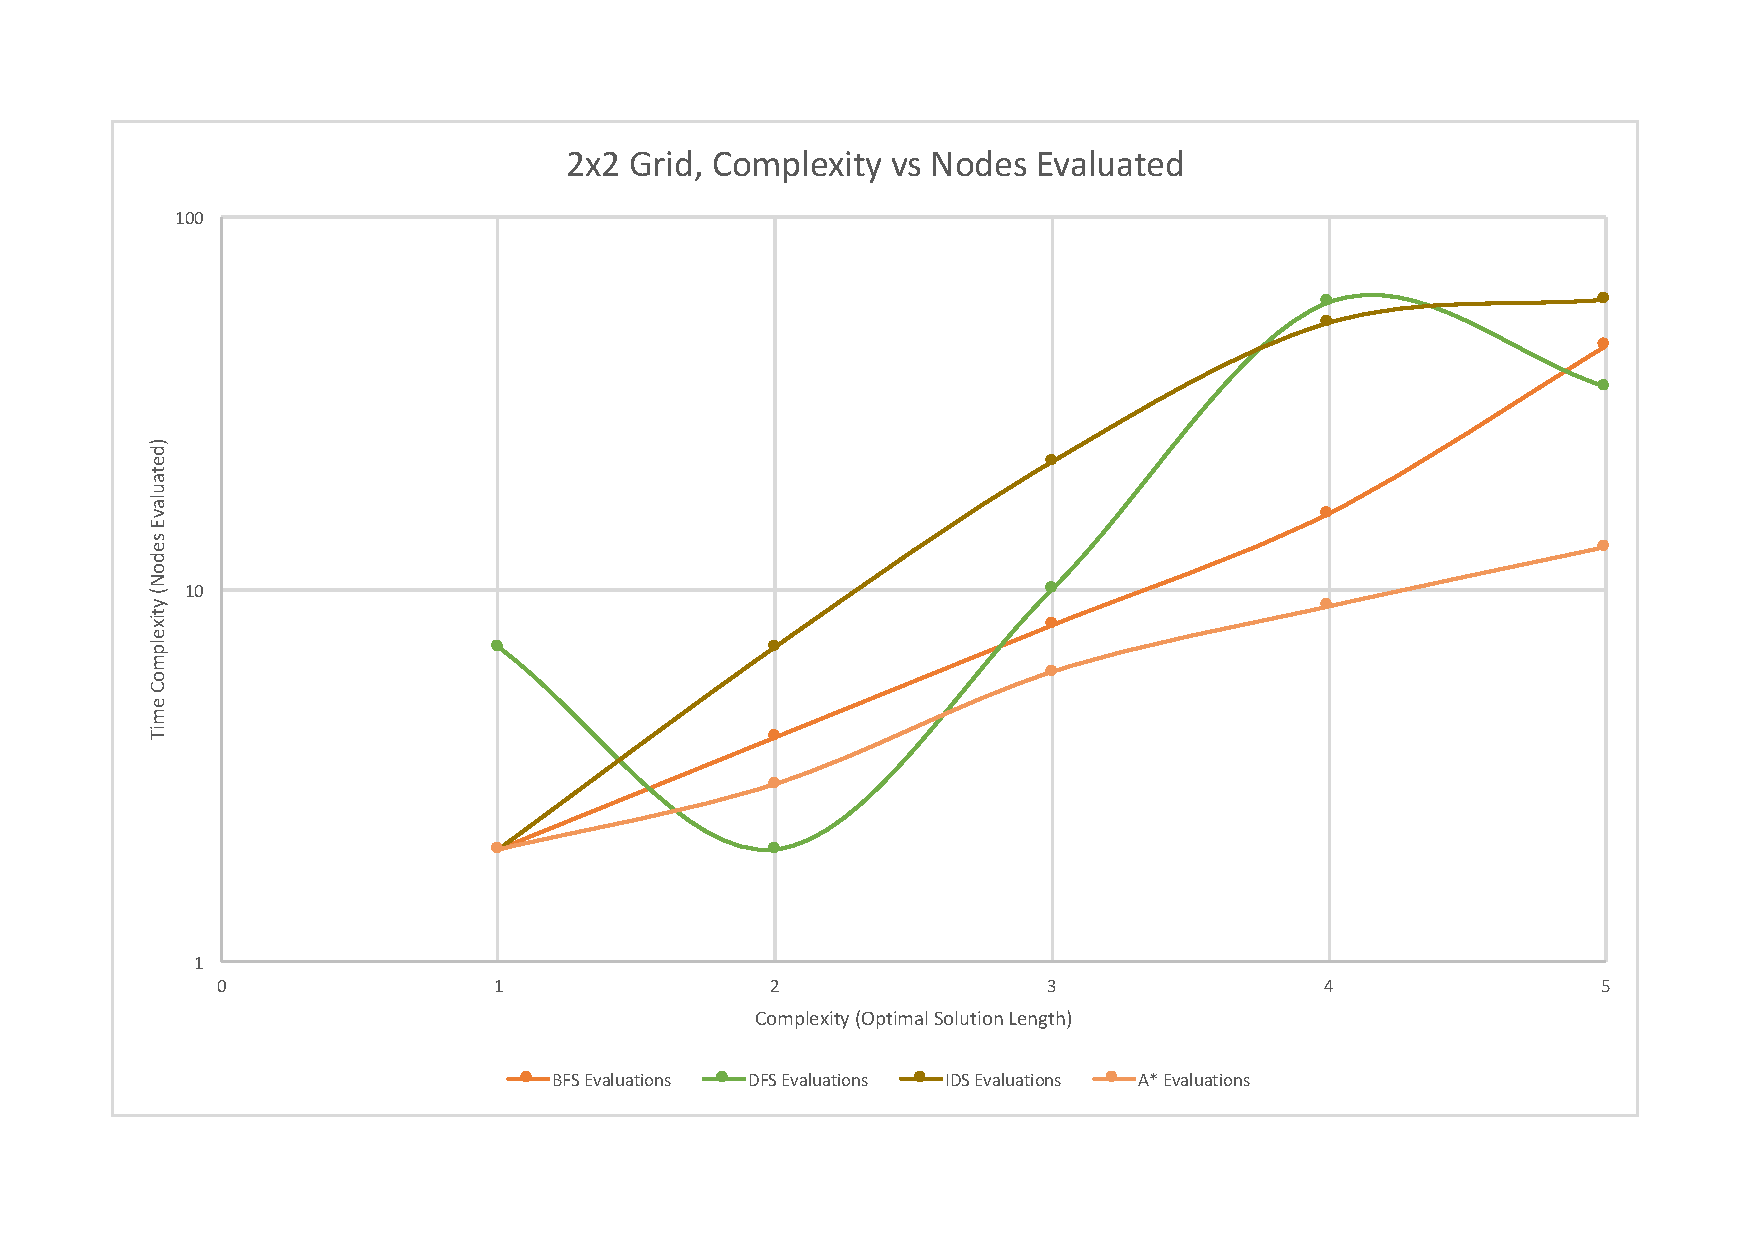
\includepdf[landscape=false,scale=0.9,angle=90,pagecommand={\section{Graphs}\subsection{2x2 Grid, Complexity vs Nodes Evaluated}\label{app:graph_2x2}}]{charts/Complexity-2x2.pdf}
  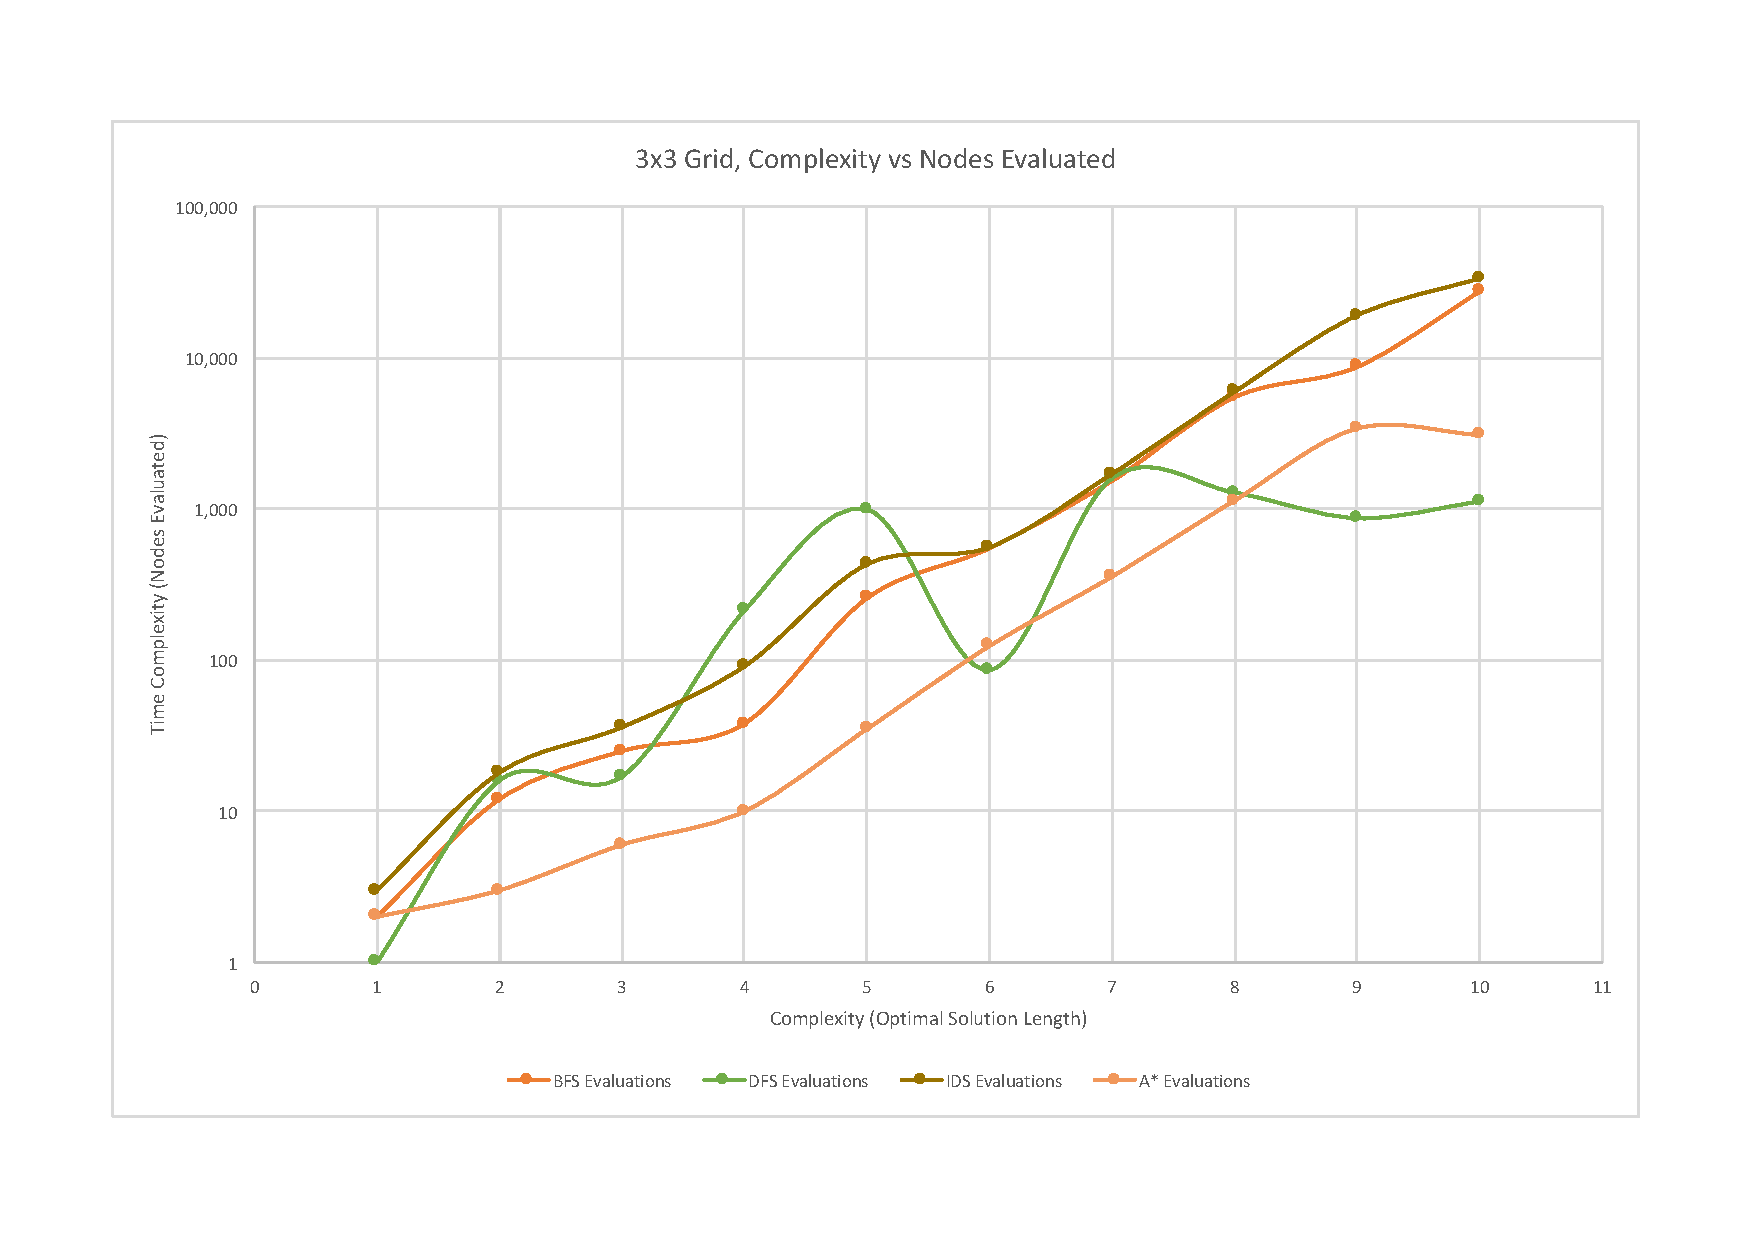
\includepdf[landscape=false,scale=0.9,angle=90,pagecommand={\subsection{3x3 Grid, Complexity vs Nodes Evaluated}\label{app:graph_3x3}}]{charts/Complexity-3x3.pdf}
  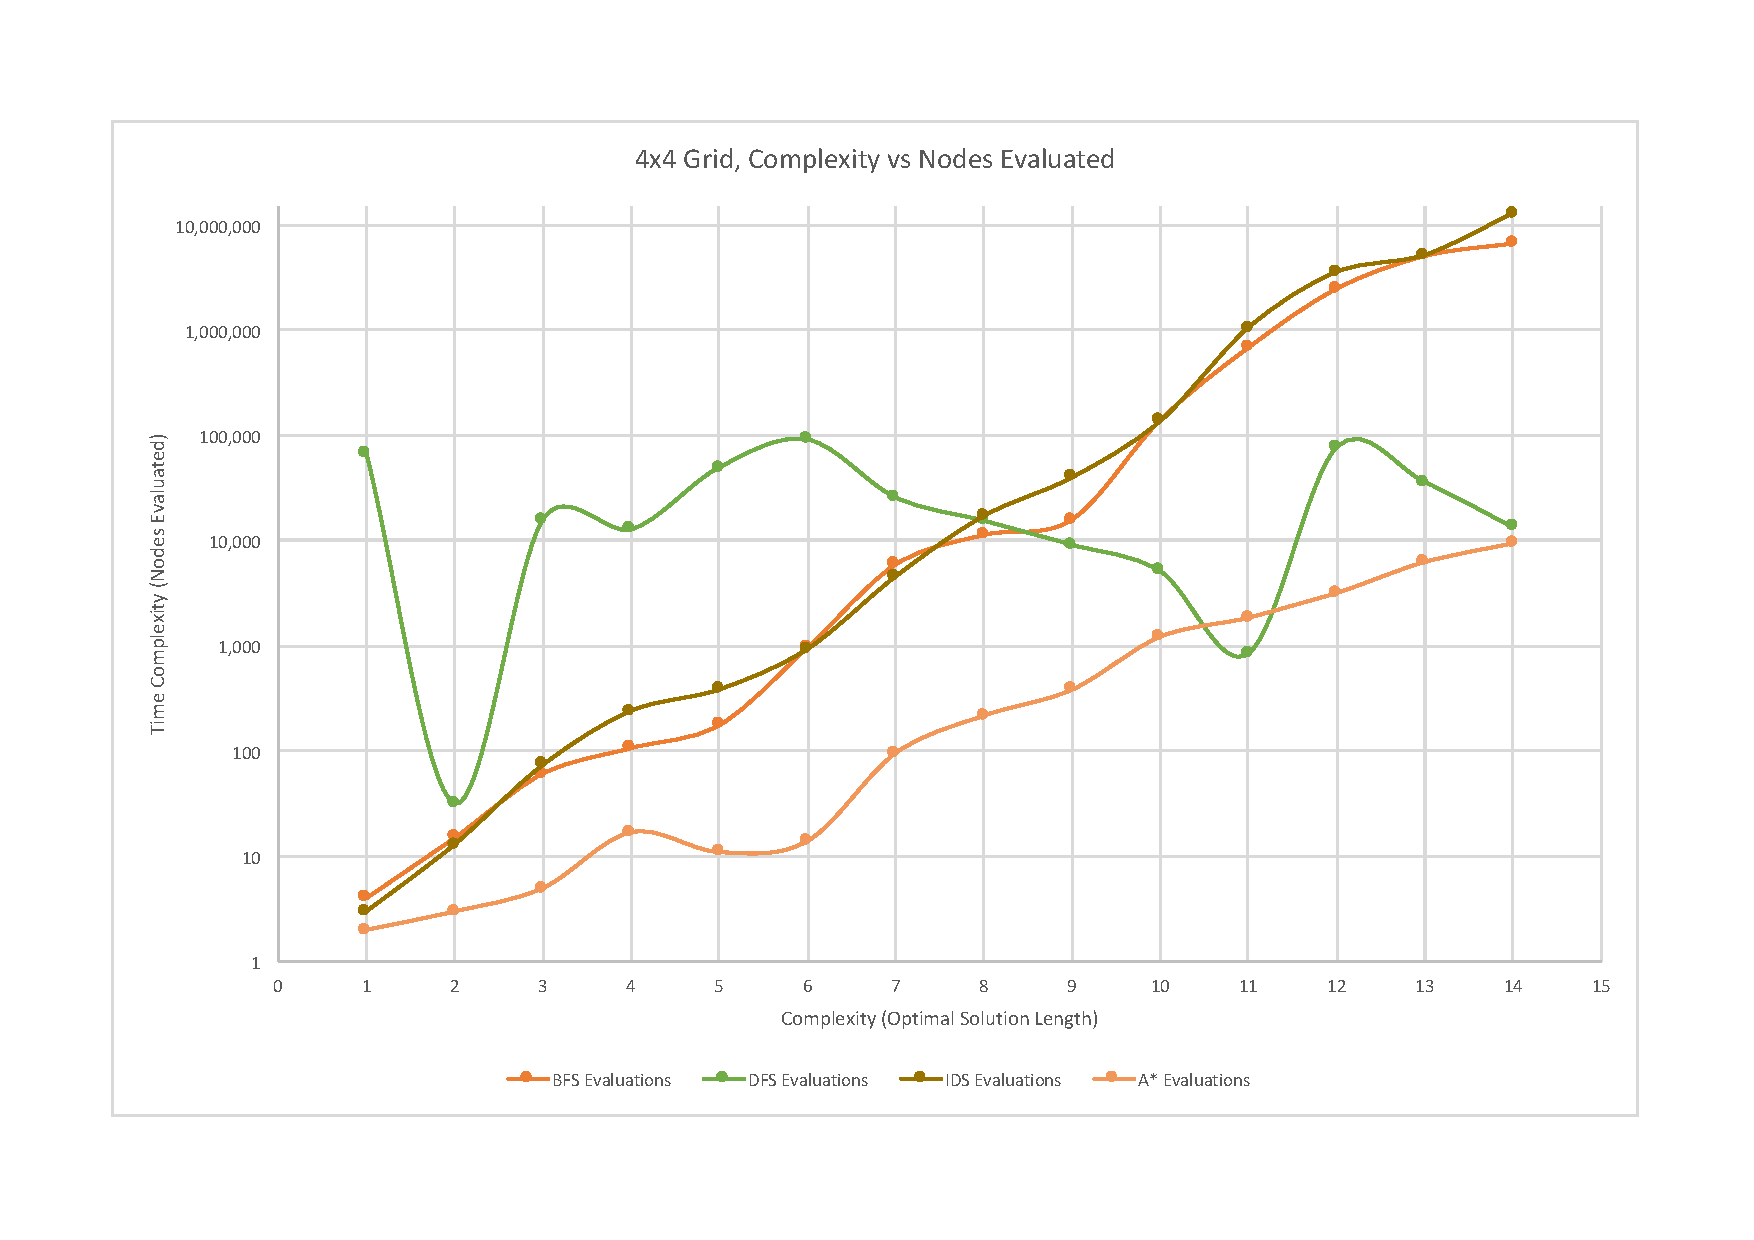
\includepdf[landscape=false,scale=0.9,angle=90,pagecommand={\subsection{4x4 Grid, Complexity vs Nodes Evaluated}\label{app:graph_4x4}}]{charts/Complexity-4x4.pdf}
  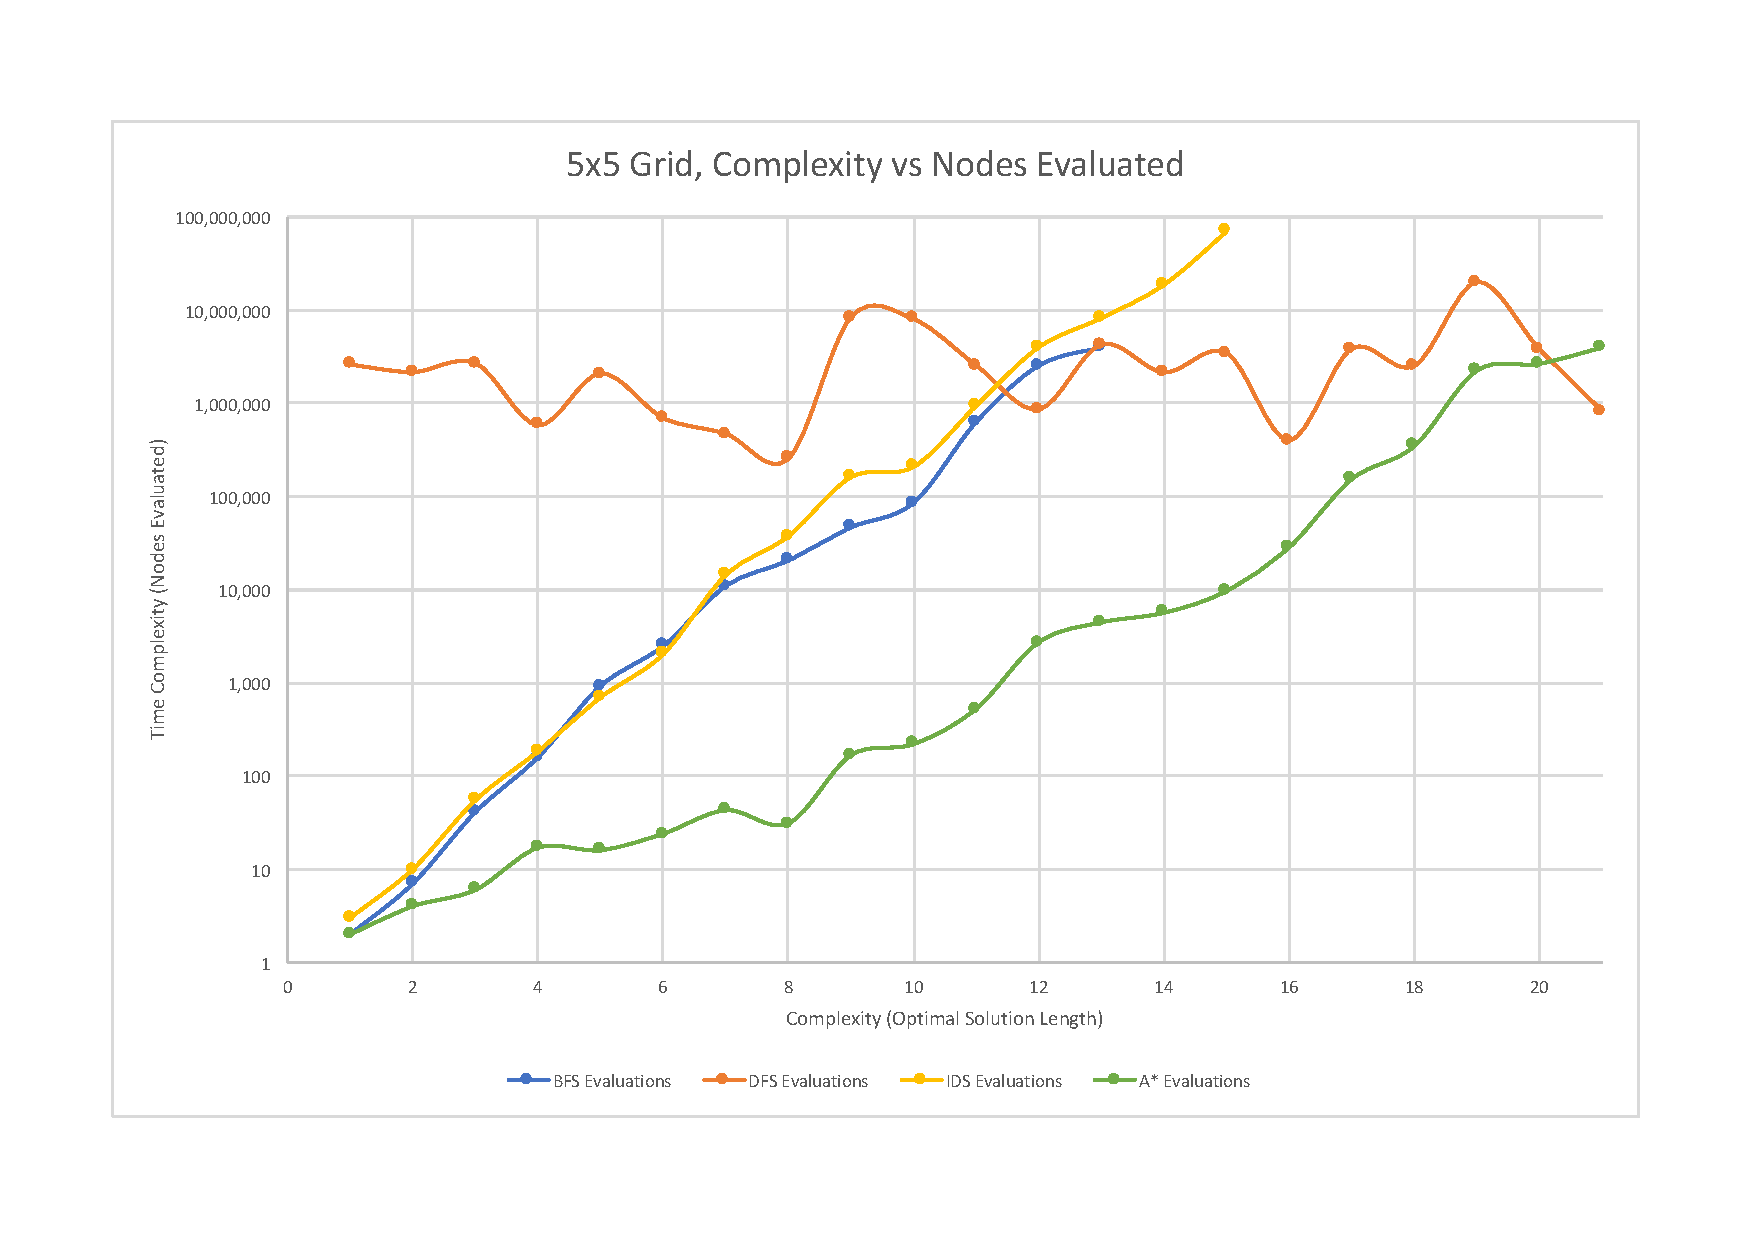
\includepdf[landscape=false,scale=0.9,angle=90,pagecommand={\subsection{5x5 Grid, Complexity vs Nodes Evaluated}\label{app:graph_5x5}}]{charts/Complexity-5x5.pdf}
  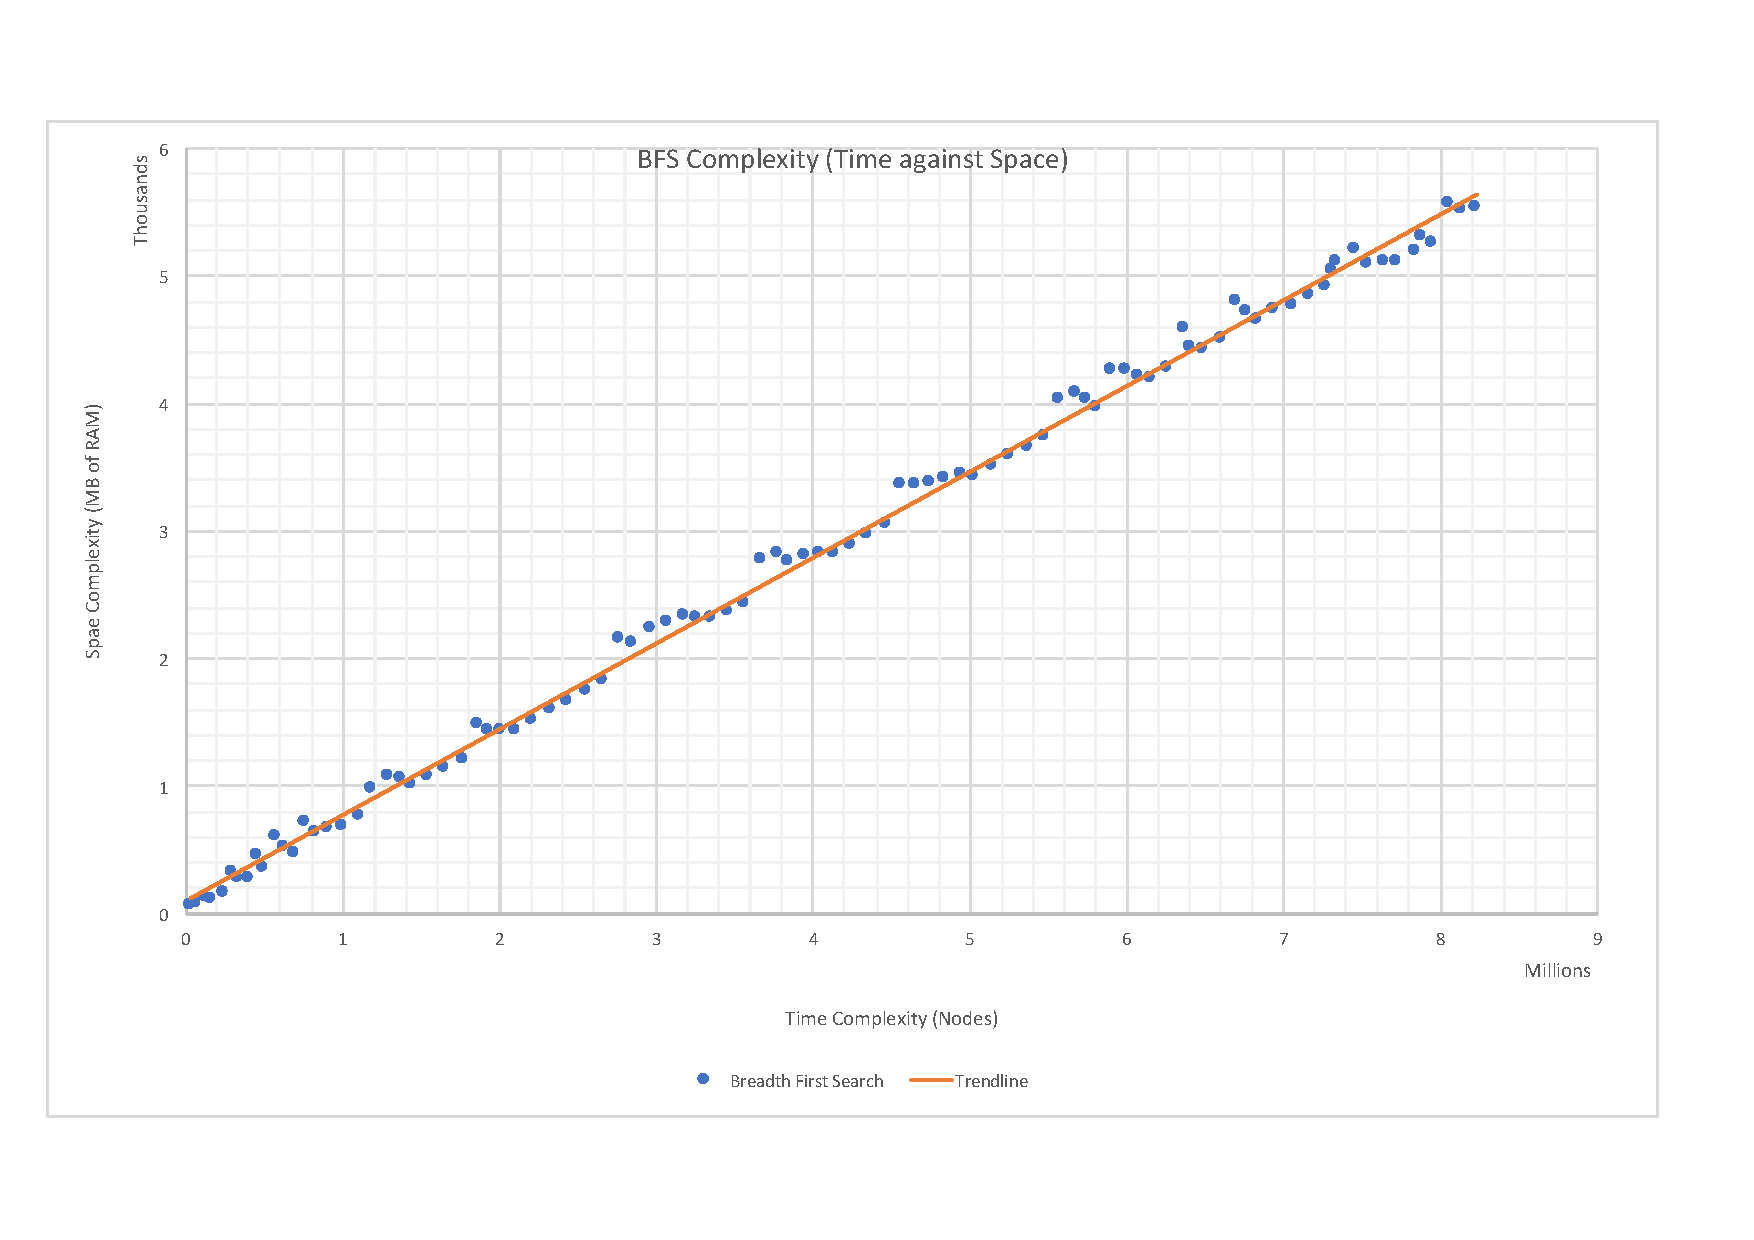
\includepdf[landscape=false,scale=0.9,angle=90,pagecommand={\subsection{BFS Complexity (Time vs Space)}\label{app:graph_bfs}}]{charts/SpaceTime-BFS.pdf}
  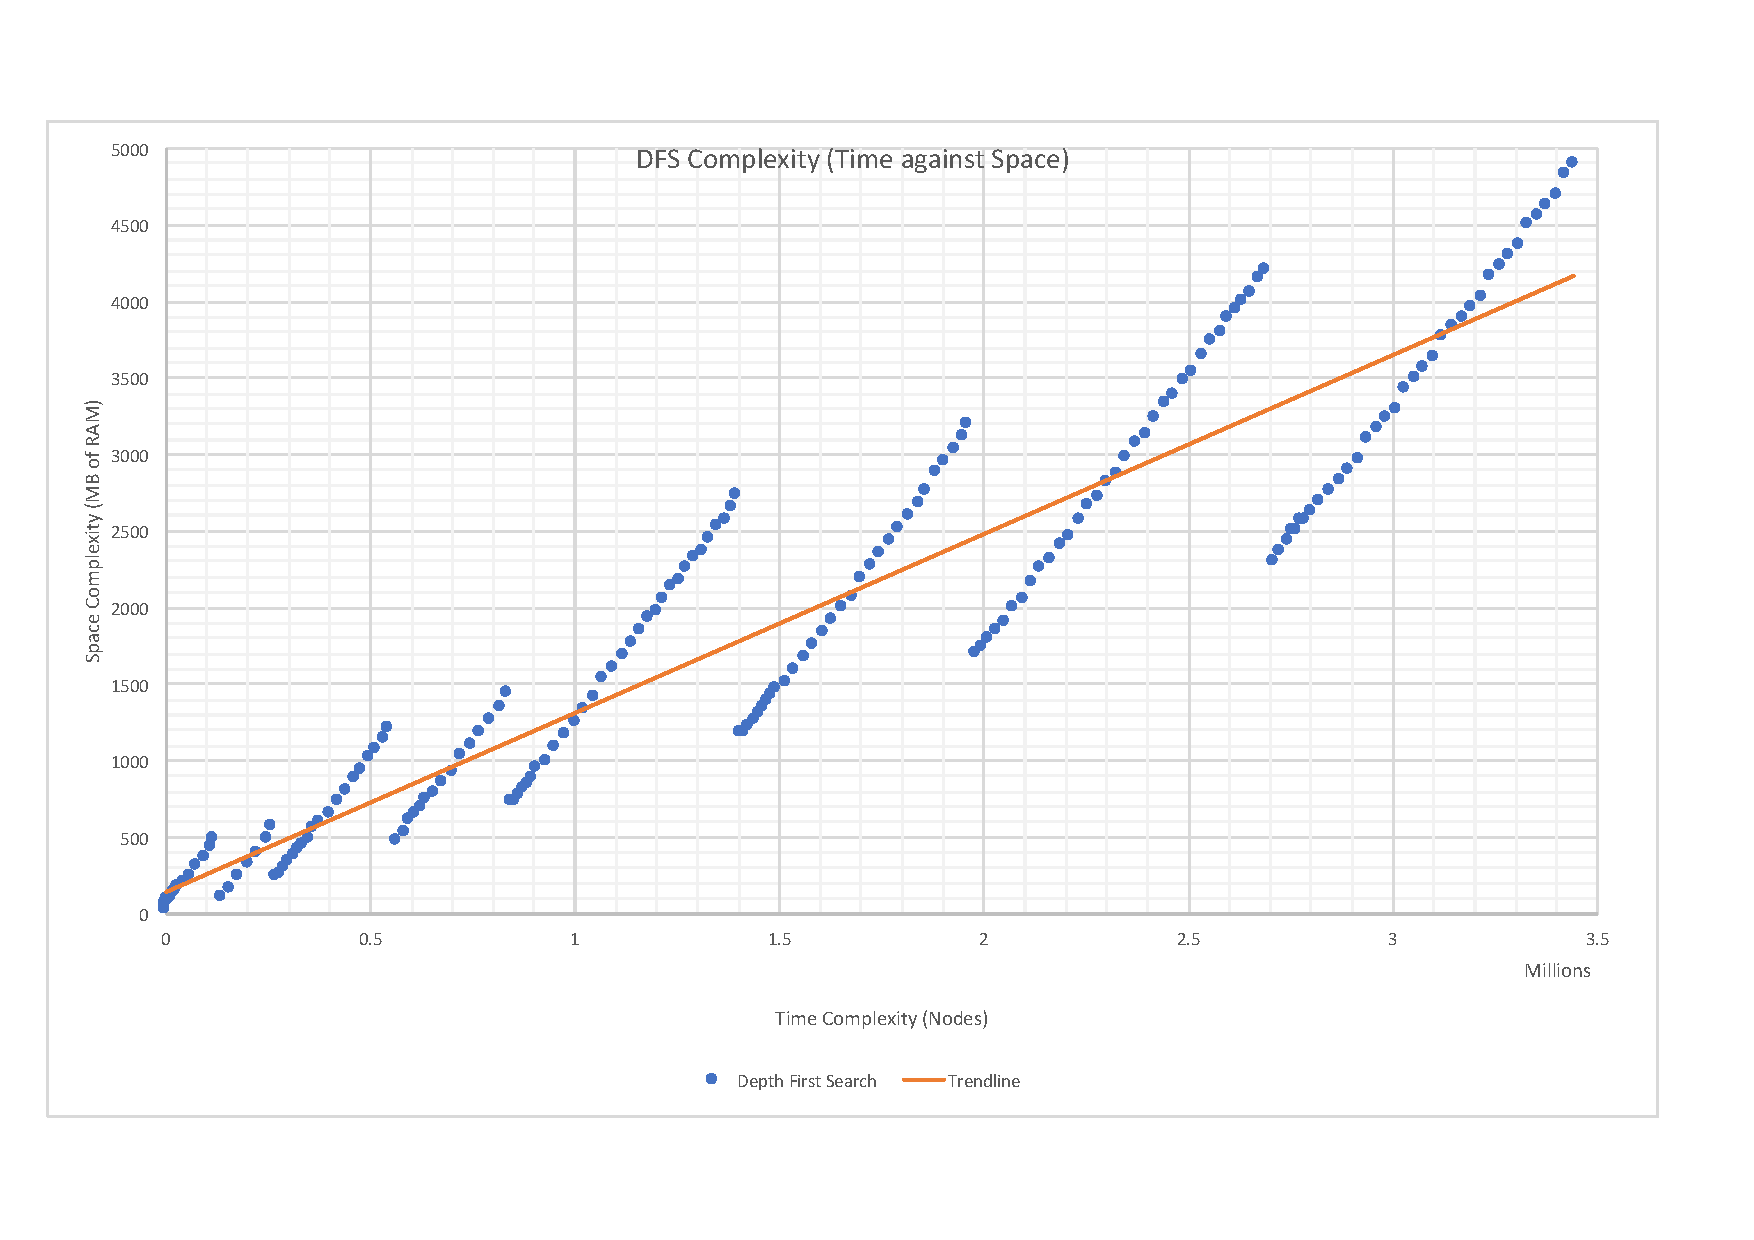
\includepdf[landscape=false,scale=0.9,angle=90,pagecommand={\subsection{DFS Complexity (Time vs Space)}\label{app:graph_dfs}}]{charts/SpaceTime-DFS.pdf}
  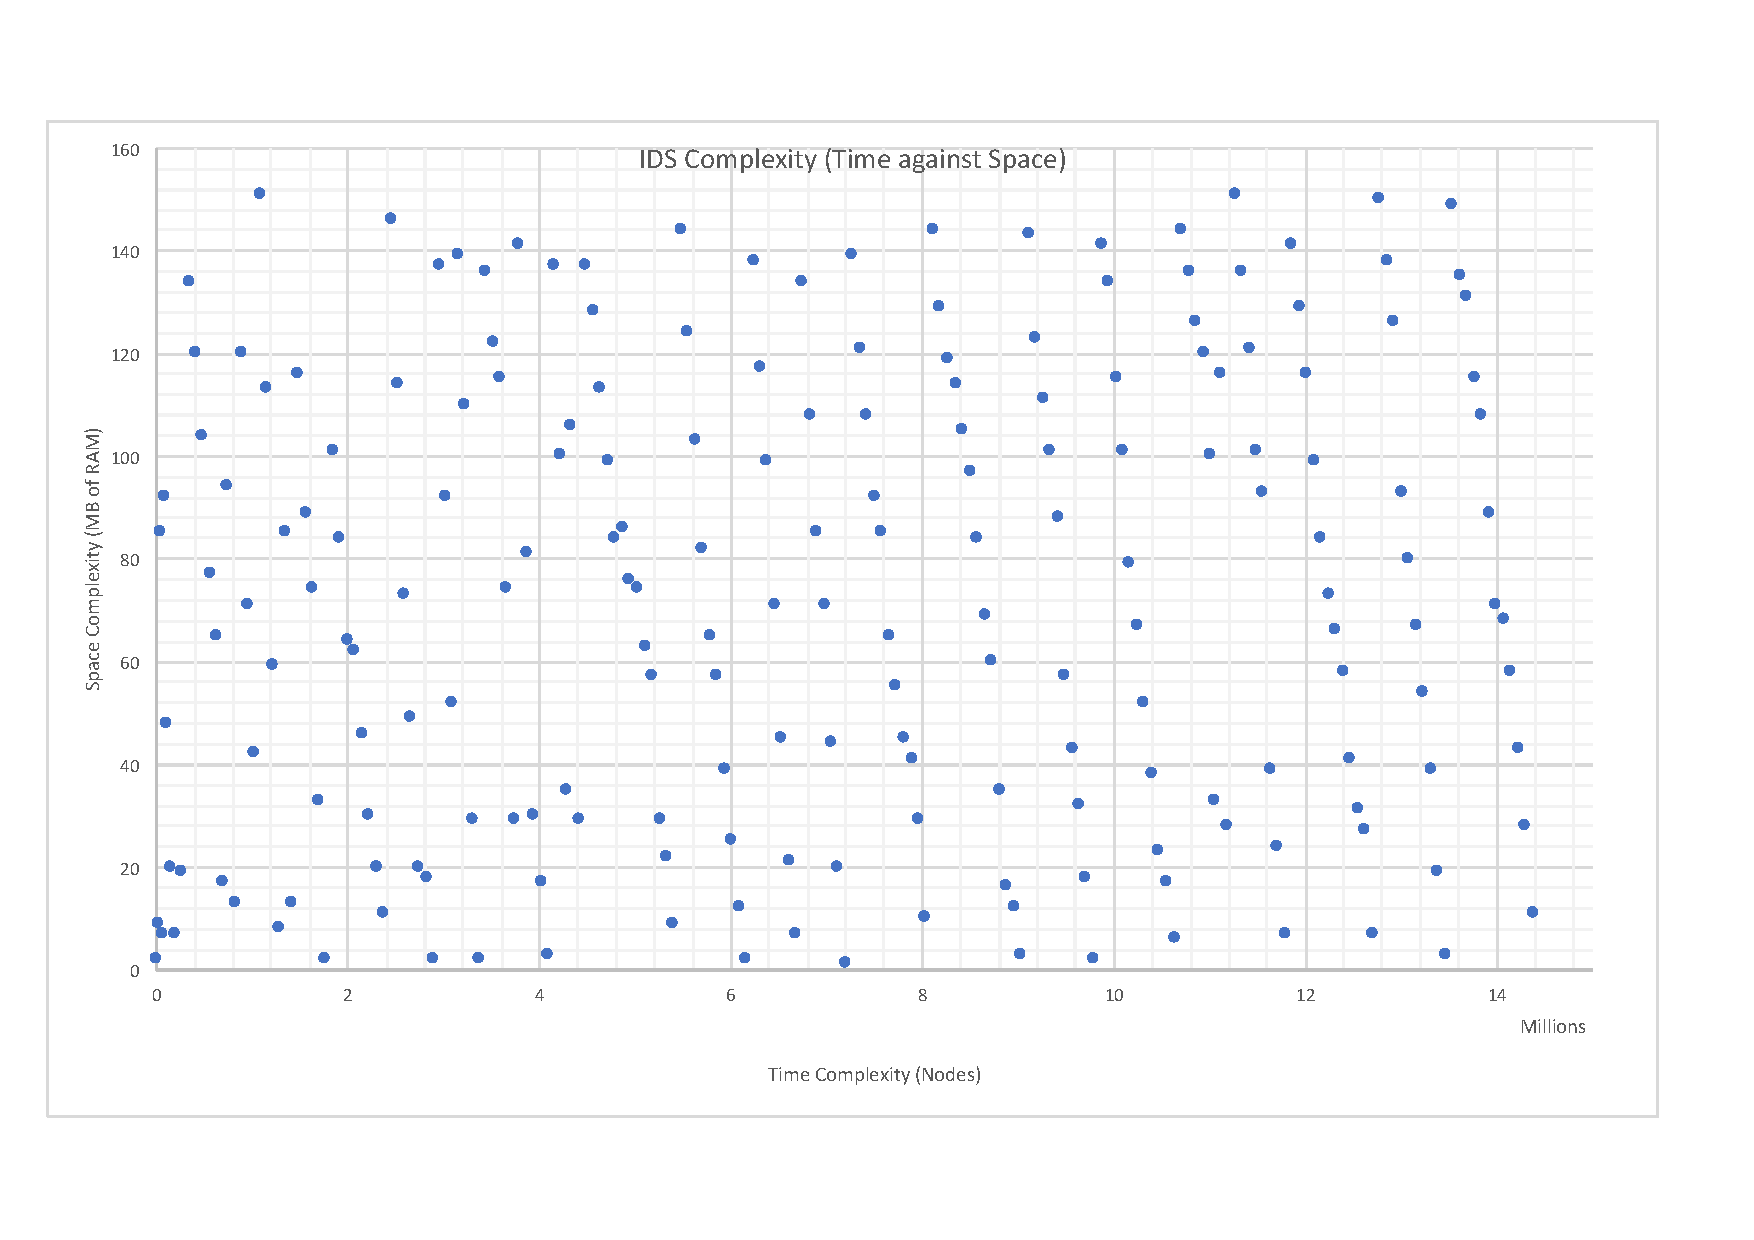
\includepdf[landscape=false,scale=0.9,angle=90,pagecommand={\subsection{IDS Complexity (Time vs Space)}\label{app:graph_ids}}]{charts/SpaceTime-IDS.pdf}
  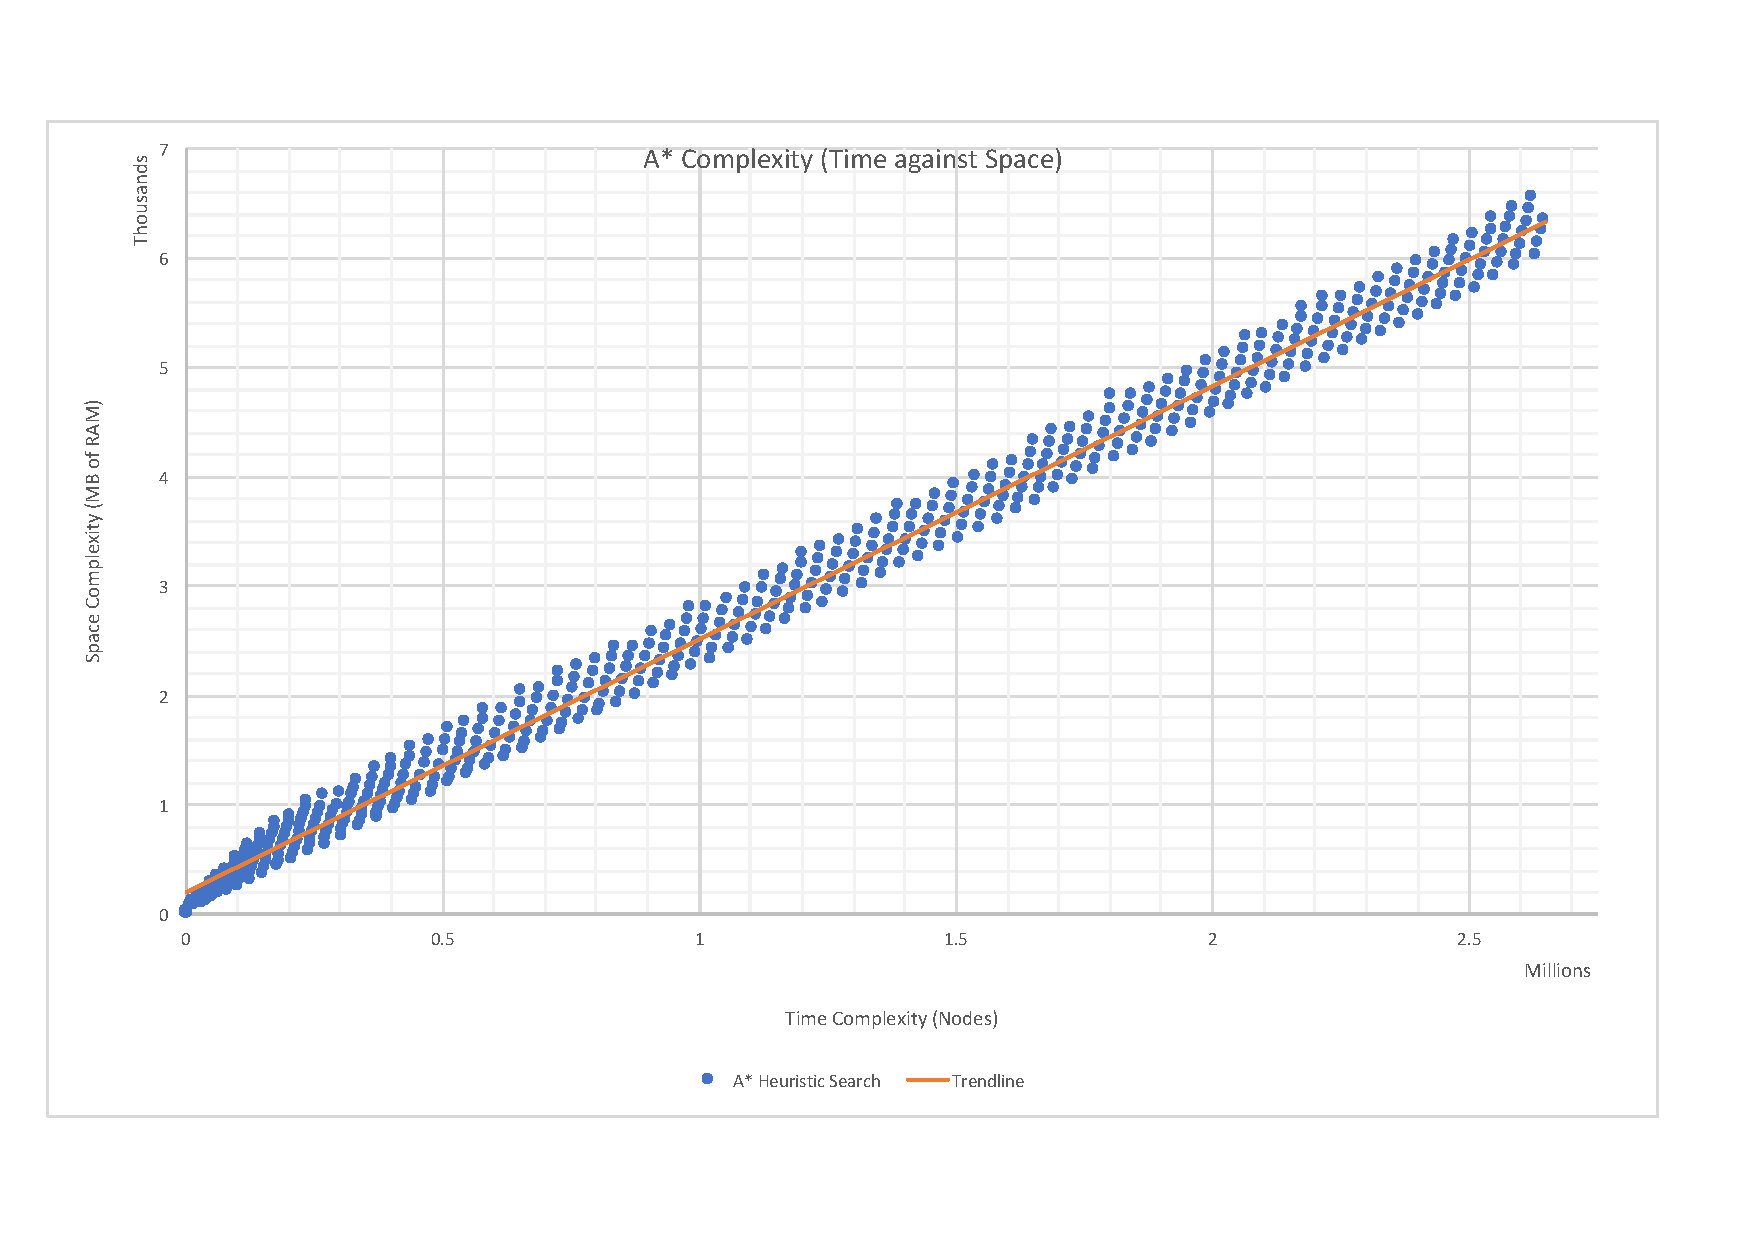
\includepdf[landscape=false,scale=0.9,angle=90,pagecommand={\subsection{A* Complexity (Time vs Space)}\label{app:graph_a*}}]{charts/SpaceTime-AStar.pdf}
\end{appendices}
\end{document}
